\documentclass[a4paper,10pt]{article}

\usepackage{fancyhdr} % clears the header and footer setting
\usepackage{graphicx} 
\usepackage{geometry}
\geometry{a4paper, left=2cm, right=2cm, top=1.5cm, bottom=3cm }
\usepackage{caption}
\usepackage{subcaption}
\usepackage{hyperref}
\usepackage{natbib}

\usepackage{etoolbox,fancyhdr,xcolor}
\newcommand{\headrulecolor}[1]{\patchcmd{\headrule}{\hrule}{\color{#1}\hrule}{}{}}
\newcommand{\footrulecolor}[1]{\patchcmd{\footrule}{\hrule}{\color{#1}\hrule}{}{}}
\renewcommand{\headrulewidth}{1pt}
\headrulecolor{red!100}%
\renewcommand{\footrulewidth}{1pt}
\footrulecolor{red!100}%

\fancyhf{}
\fancyhead[R]{
\includegraphics[width=0.25\textwidth]{nmims.png}}

\fancyfoot[C]{Nilkamal School of Mathematics, Applied Statistics & Analytics}
\fancyfoot[R]{\thepage}

\setlength{\headheight}{15mm}
\pagestyle{fancy} %This command sets the page style to fancy, applying the header and footer configurations defined above to the document pages.

\bibliographystyle{apacite}

\usepackage{times}
\begin{document}

\noindent 
\begin{center}
\textbf{{\Large Role of Green Packaging In Consumer Purchasing Decisions using Logistic Regression}} \\
\end{center}

\noindent 
\textbf{Nitya Verma,} \textit{Narsee Monjee Institute Of Management Studies, Mumbai}\\

\noindent 
\textbf{ABSTRACT: } The abstract is a summary of your research project and includes motivation, aims, methods used, (preliminary) findings and (preliminary) conclusions.  The abstract should be a stand-alone document that someone could read to get a general overview of your research project.  

Write the abstract the font shown but make sure it is no longer than about 500 words (and it must fit on a single page which includes the title, authors and keywords). The words of ‘Abstract’ and ‘Keywords’ are set in bold and full caps.  Make sure you put your correct project code in the footer. If you have two supervisors you can list both of them.  If one of them is from industry you should give their company name etc.
Please note the following rules regarding the final paper:
\begin{itemize}
    \item First page (starts with - Title, Authors, Abstract(s) and Keywords) [MANDATORY] and then follows
    \item Body of the paper (text and tables and or figures in the format shown) [MANDATORY]
    \item Notation [OPTIONAL]
    \item Appendices [OPTIONAL]
    \item References [MANDATORY]
\end{itemize}

The total length of the paper is to be no more than \textbf{14pp for 3rdyr and 19pp for 4thyr}. A cover sheet is also required in addition to the research paper. Note that the cover sheet is not included in the page limit.
\\

\noindent 
\textbf{KEYWORDS:} Keyword 1, Keyword 2 and Keyword 3. You can include a maximum of 6 keywords for indexing purposes (spaced by commas). Keywords are single words or short phrases describing the main concepts/topics covered in the paper. Sometimes only 2 or 3 keywords will suffice, but definitely no more than six.\\


\section{INTRODUCTION}

Consumers are the essence of any business. They come at the top of the development process of every business./cite(Witek2020). The phrase customer is king is valid in every venture across the globe as they make or break a business. The importance given to the customers makes it all the more crucial to understand their psyche and behaviour as that directly impacts the firms' profit and longevity. 


It's no surprise that environmental contamination is at its peak currently /cite(RaviVyas2023). An enormous bulk of this contamination comes from waste packaging. Due to the growing age of the internet, the social and environmental awareness of consumers is growing rapidly \cite{Groening2018}. People care more about the state of the world now than ever before. 

Corporate Social Responsibility (CSR) activities were made mandatory in April 2014 under the Companies Act 2013. The main aim of this modification by the Government of India was to inculcate a sense of social consciousness in the firms. The increase in environmental degradation made it all the more vital for the firms to make small changes to influence society at large, which led to the popularity of a new term known as "Green Marketing". Green Marketing came into emergence in the 1980s. It simply means the promotion, distribution, and packaging of products and services by focusing on their sustainability and ecological benefits. 

Green Marketing comes with its own set of pros and cons but the perspective matters. Looking from a broader outlook, Green Marketing has more pros than drawbacks. The positive effect it has on the environment in the long run, a better brand image, and appeal to environmentally conscious customers. It becomes crucial for organizations and businesses to pay more attention to green marketing as it plays a huge role from a competitive perspective as well. Consumers would naturally opt for environment-friendly products \cite{Groening2018}


\subsection{Green Packaging}

Green packaging is a subset of green marketing. It refers to the usage of eco-friendly packaging instead of plastics and non-biodegradable items. Ministry of Food Processing Industries published a focus paper, \cite{MOFPI2023} which gave insights on sustainable packaging. Some of the major benefits of green packaging mentioned in the paper were minimizing carbon footprint, waste reduction, and improvement in brand image. Food, normally requires plenty of packaging which in turn requires excessive materials. Paper packaging, biodegradable plastics, and compostable plastics are some of the common green packaging products.



\begin{itemize}
    \item If you want to list bullet points you can do so;
    \item This is the second point;
    \item This is a third bullet point;
    \item A fourth bullet point;
    \item But you can.
\end{itemize}   

After a list you must leave a single blank line and remember to add the indent if you are starting a new paragraph.

\subsection{Another sub-heading}

You can have as many sub-headings in a section as you want to. Note that sub-headings have a 6pt spacing after them rather than a blank line but they are preceded by a blank line. The number of sections and sub-sections is up to you, as are the titles of each of them and this will be driven by the content of your report.

\section{Methodology}

\subsection{Logistic Regression}

Logistic regression is a supervised learning technique used for classification problems. It helps in classifying data into classes on the basis of independent variables. The dependent (target) variable is binary in nature that is it has two outcomes. 
Logistic regression makes the use of sigmoid function which helps in the transformation of any real-valued number into a number between 0 and 1. Figure \ref{sigmoid} shows an S-shaped graph of a sigmoid function. 


\begin{figure}[ht]
\centering
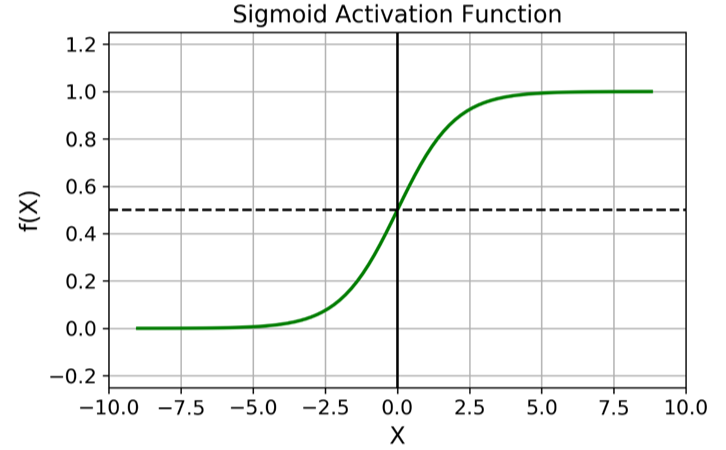
\includegraphics[height=6.6cm]{figures/sigmoid.png}
\caption{Sigmoid Function}
\label{sigmoid}
\end{figure}

(\ref{sigmoid_eq}) shows the equation of a sigmoid function where $x$ is any real-valued number which needs to be converted into a number between 0 and 1

\begin{equation}
f(x) = \frac{1}{1 + e^{-x}}
\label{sigmoid_eq}
\end{equation}

\subsection{Data}
\subsubsection{Data Collection}

The data is stimulated using Python and AI tools. An overview of the variables considered in the data was taken by going through different research papers and articles. 

\subsubsection{Data Summary}
The sample encompasses the purchase decisions made by customers regarding various products, which may or may not feature green packaging.The dataset has 330 customers and their information. 
The data consists of the following variables
\begin{itemize}

    \item Income 
    \item Age 
    \item Gender 
    \item Price of the product
    \item Type of product
    \item Green packaging (Yes/No)
    \item Purchase Decision (Yes/No)
\end{itemize}

Whether the customer purchased the product or not is the dependent variable and the rest are independent variables. 

\begin{table}[h]
\centering
\caption{Summary Statistics}
\begin{tabular}{|l|l|l|l|l|l|l|}
\hline
\textbf{Index} & \textbf{Age} & \textbf{Income} & \textbf{Gender} & \textbf{Price} & \textbf{Green Pack} & \textbf{Purchase} \\
\hline
Count & 330 & 330 & 330 & 330 & 330 & 330 \\
\hline
Mean & 40.188 & 79093.939 & 0.500 & 2305.558 & 0.545 & 0.661 \\
\hline
Std & 10.561 & 31987.012 & 0.501 & 1251.297 & 0.499 & 0.474 \\
\hline
Min & 20 & 25000 & 0 & 300 & 0 & 0 \\
\hline
25\% & 31 & 52250 & 0 & 1200 & 0 & 0 \\
\hline
50\% & 40 & 78000 & 0.5 & 2050 & 1 & 1 \\
\hline
75\% & 49 & 98000 & 1 & 3206.75 & 1 & 1 \\
\hline
Max & 60 & 160000 & 1 & 4932 & 1 & 1 \\
\hline
\label{summary_statistic}
\end{tabular}
\end{table}

Table \ref{summary_statistic} shows the summary statistic of all the variables. The average price is  2305.558 and the mean income of the customers is 79093.939. The lowest income is 25000 and the maximum income is 160000



\begin{table}[h]
\centering
\caption{Correlation Matrix}
\begin{tabular}{|l|l|l|l|l|l|l|}
\hline
 & \textbf{Age} & \textbf{Income} & \textbf{Gender} & \textbf{Price} & \textbf{Green Pack} & \textbf{Purchase} \\
\hline
\textbf{Age} & 1.00 & 0.87 & -0.07 & 0.69 & -0.17 & 0.33 \\
\hline
\textbf{Income} & 0.87 & 1.00 & -0.03 & 0.81 & -0.14 & 0.41 \\
\hline
\textbf{Gender} & -0.07 & -0.03 & 1.00 & -0.04 & -0.16 & -0.06 \\
\hline
\textbf{Price} & 0.69 & 0.81 & -0.04 & 1.00 & -0.21 & 0.35 \\
\hline
\textbf{Green Pack} & -0.17 & -0.14 & -0.16 & -0.21 & 1.00 & -0.06 \\
\hline
\textbf{Purchase} & 0.33 & 0.41 & -0.06 & 0.35 & -0.06 & 1.00 \\
\hline
\label{Correlation_matrix}
\end{tabular}
\end{table}

Table \ref{Correlation_matrix} shows the correlation among the numerical variables. It is evident from the table that the \textit{Income} of the customers and the \textit{Purchase decision} of the customers are positively correlated. 
It is also apparent that there is a negative correlation between the \textit{age} of the customers and the decision to \textit{buy} the product



\subsection{Case Analysis}


\begin{figure}[ht]
\centering
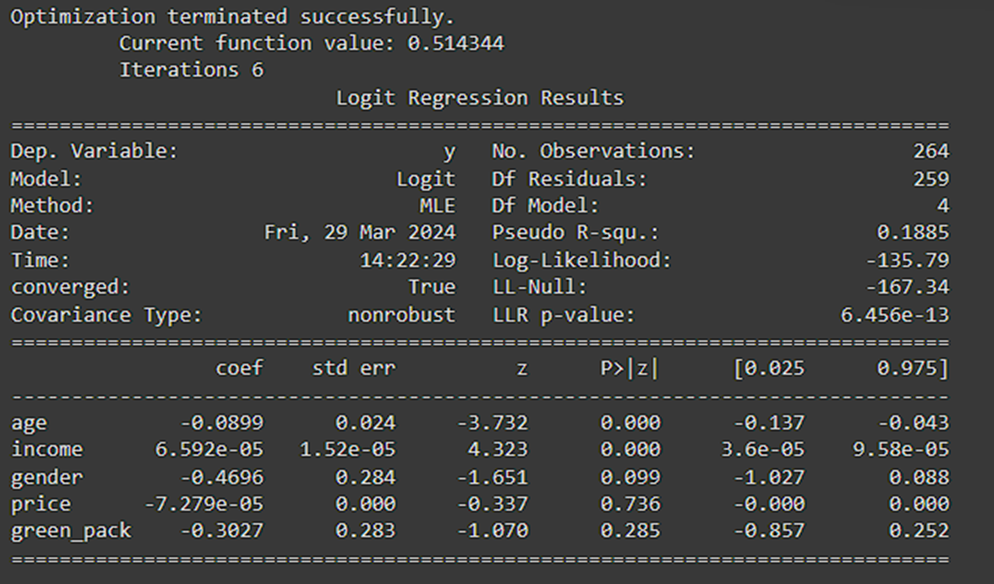
\includegraphics[height=6.6cm]{figures/coeff.png}
\caption{Summary of Logistic Function}
\label{fig_regression}
\label{summary_lr}
\end{figure}

\ref{summary_lr} shows the output of a python code. 
%complete this




\begin{figure}[ht]
\centering
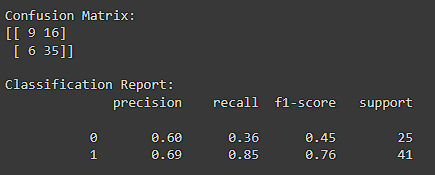
\includegraphics[height=4.5cm]{figures/class_table.png}
\caption{Classification Table}
\label{class_tab}
\end{figure}

\ref{class_tab} shows the classification table. %add labels


\begin{figure}[ht]
     \centering
     \begin{subfigure}[b]{0.45\textwidth}
         \centering
         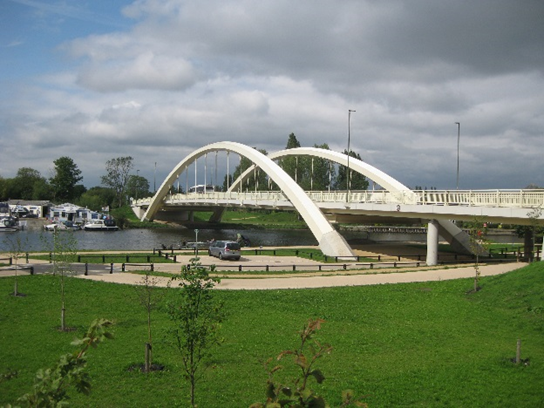
\includegraphics[width=\textwidth]{figures/fig_bridge1}
         \caption{Bridge 1}
         \label{fig_bridge1}
     \end{subfigure}
     \hfill
     \begin{subfigure}[b]{0.45\textwidth}
         \centering
         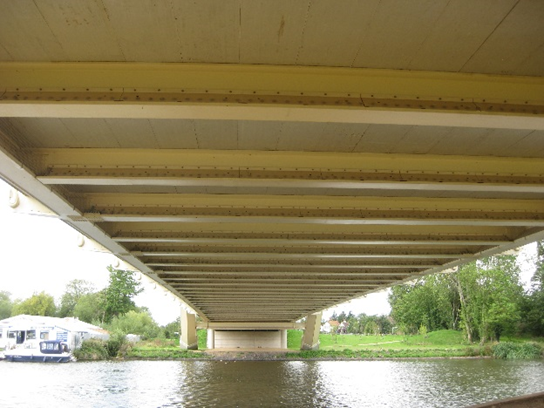
\includegraphics[width=\textwidth]{figures/fig_bridge2}
         \caption{Bridge 2}
         \label{fig_bridge2}
     \end{subfigure}
        \caption{Walton-on-Thames Bridge (a) wide shot and (b) the underside of the deck
(photos taken by P. J. Vardanega, used with permision)}
        \label{fig_twobridges}
\end{figure}




\begin{table}[h]
\begin{center}
\caption{Summary of the database (note that table captions go ABOVE THE TABLE)}
\begin{tabular}{ |l|c|l| }
\hline
 \textbf{Column heading} & \textbf{Column heading}    & \textbf{Column heading} \\ \hline 
 Table Text     & 10     & Falling head permeameter \\  \hline 
 Concrete       & 2      & Strong \\ \hline 
 Steel          & 1      & Stronger \\ \hline 
 Timber         & 3      & Weak \\ 
 \hline
\end{tabular}
\label{tab_materials}
\end{center}
\end{table}











\section{SUMMARY}

The conclusions to be drawn from this work are as follows:
\begin{itemize}
    \item 	This is a great template
\end{itemize}


At the end of the reference list no more than 15 pages should be in your ENTIRE document (including the cover sheet). Do check else a penalty will be applied!  (For students enrolled in CENGM0080 your document including the cover sheet must be no longer than 20 pages using this template).

Remember you need to submit your research paper as a PDF document! Make sure you check that all the fonts, figures and text is preserved in the layout you intend when PDF conversion is done!


\subsection{Limitations and Recommendations for further work}

For this research paper it is useful to include this section where you discuss the limitations of your work and point to future work.

\section{ACKNOWLEDGEMENTS}

Use this section to thank people who have assisted during the project – if you want. It is good form to thank your supervisor, technicians and doctoral students who have helped and anyone else who deserves a mention – but do not make it too personal. 

For example, ‘the author wishes to thank Dr X for their supervision throughout the year and also Mr G who helped build the testing rig described in this paper.’
Use this section to thank your data sources including citations to the data, weblinks, etc.

\section{APPENDIX I}

These are NOT RECOMMENDED. However, if you want to put a mathematical derivation or large data table at the back of the paper in an appendix please put it before the NOTATION LIST. 

\section{APPENDIX II}

If a second appendix is used then call the first appendix ‘APPENDIX I’ and the second ‘APPENDIX II’ and so on.

\section{NOTATION}

This section is optional. If you have few equations it may be better to simply define all the variables in the text as shown. For highly mathematical papers this section is very helpful for the reader. Note that this section heading is not numbered. Please put the following statement in italics before the notation list:

\textit{The following acronyms and symbols are used in the work described in this paper:}

\textbf{Acronyms}

BSI	 British Standards Institute

\textbf{Symbols}

\textit{Latin}

$A$ = a constant

\textit{Greek}

$\gamma$ = shear strain



\fontsize{8}{9}\selectfont
\bibliography{ResearchPaperBib}



\clearpage



\end{document}